\documentclass{article}
% translate with >> pdflatex -shell-escape <file>

% This file is used as unit test for pgfplots, copyright by Christian Feuersaenger.
% 
% See
%   http://pgfplots.sourceforge.net/pgfplots.pdf
% for pgfplots.
%
% Any required input files (for <plot table> or <plot file> or the table package) can be downloaded
% at
% http://www.ctan.org/tex-archive/graphics/pgf/contrib/pgfplots/doc/latex/
% and
% http://www.ctan.org/tex-archive/graphics/pgf/contrib/pgfplots/doc/latex/plotdata/

\usepackage{pgfplots}
\pgfplotsset{compat=newest}

\pagestyle{empty}

\begin{document}

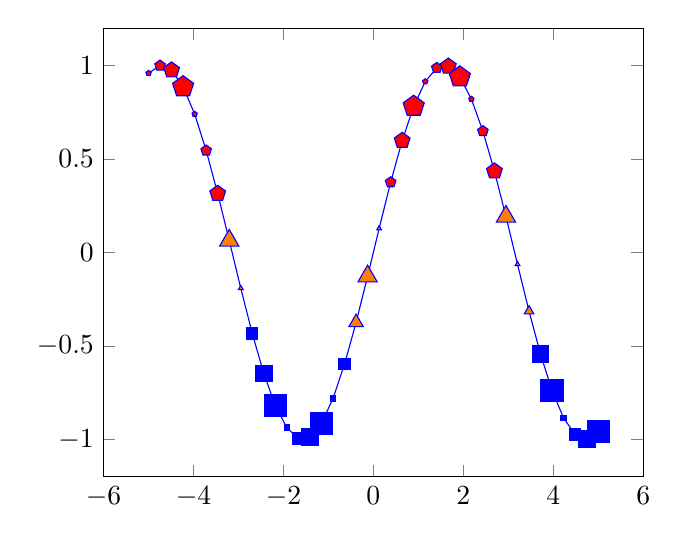
\begin{tikzpicture}
	\begin{axis}[
		scatter/@pre marker code/.code={%
			\ifdim\pgfplotspointmetatransformed pt<300pt
				\def\markopts{mark=square*,fill=blue}%
			\else
				\ifdim\pgfplotspointmetatransformed pt<600pt
					\def\markopts{mark=triangle*,fill=orange}%
				\else
					\def\markopts{mark=pentagon*,fill=red}%
				\fi
			\fi
			\expandafter\scope\expandafter[\markopts,mark size=\perpointmarksize]
		},%
		scatter/@post marker code/.code={%
		   \endscope
		},
		visualization depends on={1+mod(\coordindex,4) \as \perpointmarksize},
	]

	\addplot+[scatter,scatter src=y,
		samples=40]
		{sin(deg(x))};

	\end{axis}
\end{tikzpicture}
\end{document}
